\section{Overview} \label{sec:overview}

\begin{figure*}[t!] 
     \centering 
     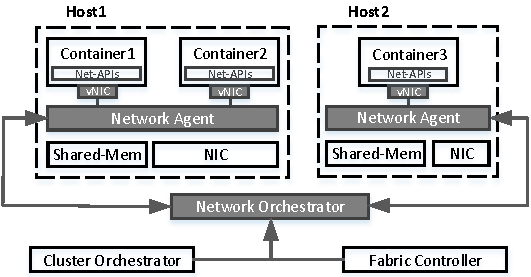
\includegraphics[width=7in]{figures/system-arch.pdf} 
    \caption{\label{fig:sysarch} The overall system architecture of exsiting overlay network and \sysname. Gray boxes are building blocks of~\sysname.} 
\end{figure*} 

In this section, we discuss the key insights to achieve a high network
performance with a little less strict isolation and without sacrificing portability of containers. We also introduce the overall architecture 
of \sysname. 

%This section presents the high-level design of \sysname. We introduce
%the requirements and concerns in the designs of control-plane, data-plane
%and network access layer, and explain what design choices \sysname makes 
%and what the reasons are behind these design choices.

\subsection{Insights for high network performance}

Container deployments opt for overlay-based networking since it is most
portable: a container does not have to worry about where the other endpoint is.
For example, in Figure~\ref{fig:sysarch}(a), Container~1 and Container~3 cannot
distinguish whether Container~2 is on Host~1 or Host~2, if only Container~2
keeps its overlay IP address (2.2.2.2) and the overlay routers know how to
route packets to this IP. 

Existing overlay-based container networks sacrifice performance for 
the good portability, because traffic needs to go through a deep software 
stack, as shown in Figure~\ref{fig:sysarch}(a). 
The key to achieve a high performance and low overhead overlay network for
containers is bypassing the performance bottlenecks, including bridges, software
routers and host OS kernel, on data-plane. Given that containers are essentially
processes, the communication channels provided by IPC and hardware offloading
techniques give us numerous hammers to build a better container network. For
instance, containers within a single host (like Container~1 and Container~2 in
Figure~\ref{fig:sysarch} (a) 
can communicate via shared-memory, and overlay routers
in different hosts can talk via RDMA (or DPDK), which helps to bypass performance
bottlenecks. Note that communication paradigms like shared-memory and RDMA 
sacrifice the isolation of containers. However, since in most cases
containers are from the same application deployed by a single tenant, they
have trust with each other and have the incentive to trade a little isolation
for a huge boost in performance.

Generally, one container should decide how to communicate
with another according to the latter's location for high networking performance. 
There are two issues to realize this key idea: (1) How to discover the real-time locations of containers; (2) How to enable containers
to use different mechanisms to communicate with different peers.

One way is to solve these two issues is merely depending on containers themselves:
one container needs to exchange location information with another one and
agree on a communication mechanism to use. Nonetheless, this method will 
break the portability of containers, e.g. container locations are never transparent, and will also make the programing of applications extremely 
complicated. 

Instead, we take an alternative approach: using a (conceptually) centralized orchestrator to decide how containers communicate, and keeping the container locations and the 
actual
communication mechanisms transparent to containers. Our key insight is that since currently most of the container clusters are managed by centralized cluster orchestrator (e.g. Mesos, Docker Swarm, etc.)\footnote{They can easily be deployed on private bare-metal clusters or cloud VM clusters without any special supports from cloud providers.}, the information about the location of the other endpoint
can be easily obtained by querying the orchestrator. By leveraging this
information, we can choose the right communication paradigm for the specific
scenario. Furthermore, all of the complexity of communication mechanism selection
and execution can be hidden from the application
by bundling it into a customized network library supporting standard 
network APIs.
Next, we sketch the architecture of our solution.

\subsection{The architecture of FreeFlow}

Figure~\ref{fig:sysarch}(a) shows the architecture of existing overlay networking
solutions for containers. Each container has a virtual NIC that is attached to
the overlay router of the host via software bridge. Different overlay routers
exchange routing information and build routing tables via standard routing 
protocols, such as BGP. The fabric build by virtual NICs, bridges, overlay routers and physical NICs of hosts and host network is the actual data-plane for
packets traversing the overlay from container to another one. Inside each container, applications leverage standard network APIs to utilize the network, and the API calls are executed by network libraries, such as \texttt{libsocket} for Socket API, and \texttt{libibverbs} for RDMA Verbs API.

\sysname is not designed and built from scratch. Instead, it reuses many
control-plane features like IP allocation and routing in the existing solution.
However, \sysname modify multiple existing modules in the networking stack
to achieve a smarter and more efficient data-plane.

Figure~\ref{fig:sysarch}(b) shows the overall architecture of \sysname.
The gray boxes in Figure~\ref{fig:sysarch}(b) presents the three kinds of
building blocks of \sysname: network orchestrator, customized overlay router and
customized network library.
\begin{itemize}

\item Network orchestrator is a central place which stores the realtime locations
of each container in the cluster. 

\item We build \sysname's overlay routers based
on existing overlay routers. There are two new features added by \sysname:
(1) the traffic between routers and its local containers goes through shared-memory instread of software bridge; and (2) the traffic between different
routers is delivered via kernel bypassing techniques, e.g. RDMA or DPDK, if
the hardware on the hosts are capable.

\item \sysname's network library is the core component which decides which
communication paradigm to use. It supports standard network programming APIs,
e.g. Socket for TCP/IP, MPI and Verbs for RDMA, etc., and keeps pulling
the newest container location formation from the network orchestrator. 


\end{itemize} 

The architecture enable the possibility to make traffic among containers flow
through an efficient data-plane: shared-memory for intra-host cases and shared-momory plus kernel bypassing networking for inter-host cases.

However, we have two challenges to achieve \sysname's simple vision.
First of all, the network library of \sysname should naturely support
multiple standard network APIs for transparency and backward compatibilities;
Second, for inter-host cases, overlay routers should connect the shared-memory
channel with local containers and the kernel bypassing channel between physical NICs to avoid overhead caused by memory copying. In next section, we will propose
the design of \sysname which can addresses the challenges.
